\chapter{Progettazione e codifica}
\label{cap:progettazione-codifica}

\intro{Questo capitolo tratta della fase di progettazione e della fase di codifica dell'app, riportando tutto quello che è stato fatto e le difficoltà incontrate.}\\ 

\section{Progettazione}
\label{sec:progettazione}

\subsection{Struttura dell'app}

Dopo una prima parte di stage, dove ho studiato le tecnologie riportate al \hyperref[sec:tecnologie]{secondo capitolo}, ho pensato come sviluppare l'applicazione richiesta.\newline
Di prassi, in RiskAPP si utilizza Figma per poter avere una idea più chiara del lavoro che si desidera fare, quindi per prima cosa ho progettato la grafica e la struttura dell'app con l'aiuto di questo software di progettazione.\newline
Avendo una idea visiva, questo rendeva più facile spiegare al mio tutor come pensavo di impostare l'applicazione, andando poi a modificare e sistemare in base alle esigenze dell'azienda.\newline
\newline
Nella Figura \ref{fig:schermatefigma} ci sono tre schermate progettate in Figma, ovvero le schermate \textbf{Utente}, \textbf{Impostazioni} e infine \textbf{Home}.\newline
Dai \emph{mockup} capiamo che la struttura delle pagine è la seguente:
\begin{itemize}
    \item una barra superiore, dove è possibile eseguire una o due azioni;
    \item una schermata con le informazioni interessate;
    \item una barra inferiore che permette di navigare tra le schermate, fatta eccezione per la schermata \textbf{Impostazioni} che non ha questa barra.
\end{itemize}
Tramite la barra inferiore è possibile navigare tra le schermate:
\begin{itemize}
    \item \textbf{Home}, dove sarà visibile la \emph{\gls{cassacomuneg}}, la \emph{\gls{quotastornatag}} dell'utente e infine il piatto del giorno (successivamente cambiato in \emph{Proposte del giorno} per permettere la scelta di più piatti dal menu);
    \item \textbf{Spese}, che permette di visualizzare tutte le transazioni di tutti gli utenti e aggiungere delle nuove transazioni o eliminarle;
    \item \textbf{Menu}, dove è possibile consultare i piatti, aggiungerli oppure proporli come possibili piatti del giorno;
    \item \textbf{Utente}, la visualizzazione cambia tra utente semplice e utente amministratore. Quest'ultima è stata modificata durante la fase di codifica, ma principalmente serve per visualizzare e modificare le proprie presenze o, nel caso dell'amministratore, visualizzare e modificare le presenze degli stagisti o della \emph{\gls{quotapastog}}.
\end{itemize}
\begin{figure}[!h]
    \centering 
    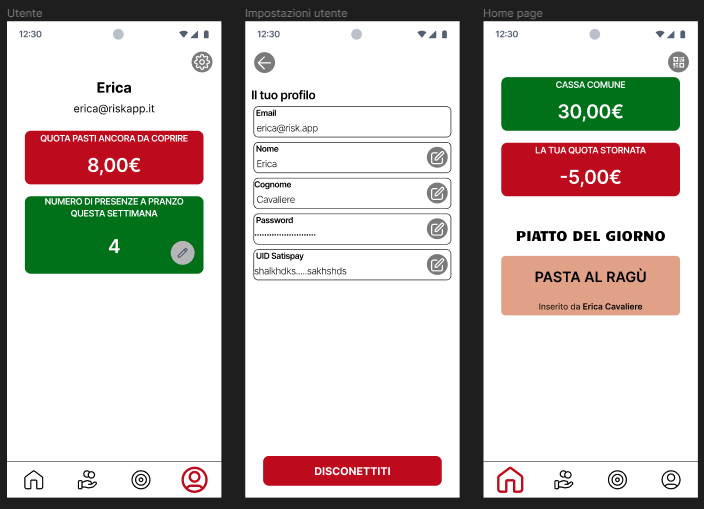
\includegraphics[width=0.9\columnwidth]{figma/esempi} 
    \caption{Alcune schermate progettate in Figma}
    \label{fig:schermatefigma}
\end{figure}
La schermata \textbf{Impostazioni} è raggiungibile attraverso la schermata \textbf{Utente}, andando a toccare l'icona ad ingranaggio posta nella barra superiore.\newline
Da \textbf{Impostazioni} è possibile modificare i dati dell'utente oppure permettere all'utente di disconnettersi dalla sessione corrente.\newline
\newline
Sono state create diversamente anche le finestre \textbf{Accedi} (Figura \ref{fig:accedifigma}) e \textbf{Registrati} (Figura \ref{fig:registratifigma}).\newline
In queste due schermate non sono presenti barre superiori o inferiori, ma solo una serie di campi da compilare e il pulsante verde Accedi o Registrati.\newline
\textbf{Accedi} è la prima schermata che vede l'utente quando entra nell'app per la prima volta; per passare alla schermata \textbf{Registrati} bisogna toccare il link presente sotto al pulsante Accedi, dove è scritto il messaggio "\emph{Sei nuovo? REGISTRATI}".\newline
Per ritornare alla schermata \textbf{Accedi}, il procedimento è analogo, ovvero si tocca il link presente sotto il pulsante Registrati, dove è riportato il messaggio "\emph{Hai già un account? ACCEDI}".\newline
Invece, per andare in \textbf{Home}, bisognerà compilare correttamente i campi e poi toccare il pulsante verde presente.\newline
\newline
In \textbf{Accedi} è presente il messaggio "\emph{Hai dimenticato la password?}", questo doveva contenere un link che permetteva all'utente di recuperare la propria password, funzionalità prima prevista, poi ritenuta non più necessaria.\newline
%qui poi si dovrà riportare le schermate a 0.7 in base all'introduzione ---------------------------------------------------------------------------------------------------------------------------------------------------------------------
\begin{figure}[!h] 
    \centering 
    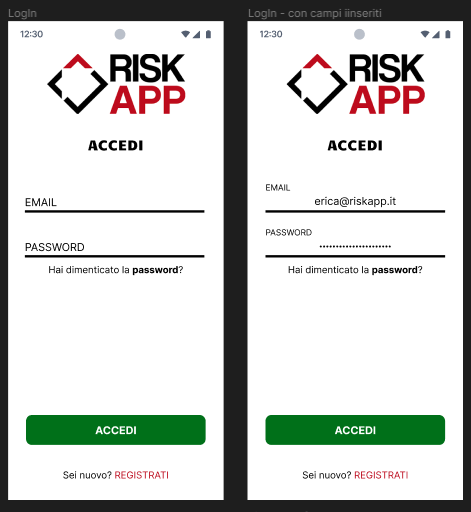
\includegraphics[width=0.6\columnwidth]{figma/accedi} 
    \caption{Schermata Accedi progettata in Figma}
    \label{fig:accedifigma}
\end{figure}
\begin{figure}[!h] 
    \centering 
    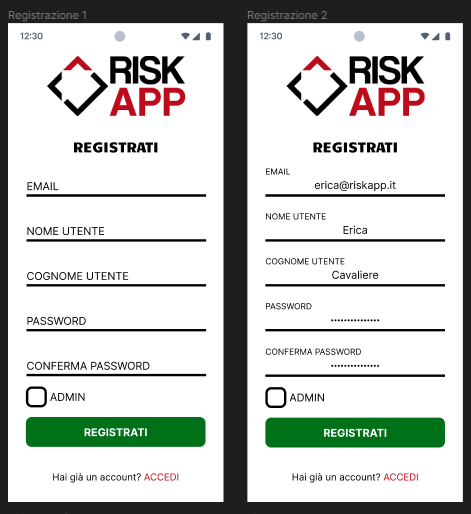
\includegraphics[width=0.6\columnwidth]{figma/registrati} 
    \caption{Schermata Registrati progettata in Figma}
    \label{fig:registratifigma}
\end{figure}
%Come è già stato detto, sono state fatte diverse modifiche in fase di progettazione, alcune modifiche sono state fatte perchè non rispettavano le idee del proponente, altre perchè non avevano utilità, come il recupero password appena accennato, altre modifiche sono state fatte anche a livello grafico, perchè non permetteva all'utente di capire che cosa poteva fare.\newline
%Per questo sono state fatte delle modifiche anche ai componenti utilizzati (nella figura \ref{fig:conteinerfigma} ci sono i \emph{component} creati per il \emph{mockup}), pure le icone dei pulsanti, che servivano solo a livello dimostrativo.
%\begin{figure}[!h] 
%    \centering 
%    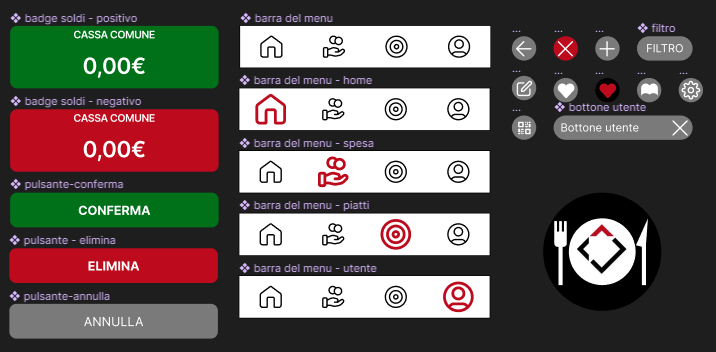
\includegraphics[width=0.9\columnwidth]{figma/container} 
%    \caption{Alcuni pulsati e icone progettate in Figma}
%    \label{fig:conteinerfigma}
%\end{figure}

\newpage

\subsection{Database}
Per quanto riguarda la base di dati (Figura \ref{fig:database}), ho pensato a una struttura semplice, mettendo al centro l'utente che può inserire dei piatti, delle transazioni oppure segnare le proprie presenze.\newline
Si è poi pensato ad un'entità isolata, che ha il solo scopo di contenere le variabili globali, ovvero la \emph{\gls{cassacomuneg}}, la \emph{\gls{quotapastog}} e la \emph{\gls{quotastornatag}} degli stagisti.\newline
Per quanto riguarda gli stagisti, inizialmente si pensava se considerarli come un utente oppure se rappresentarli come un'altra entità; alla fine, è stato deciso di lavorare in modo diverso, dato che gli stagisti si ipotizza che non utilizzino l'app.\newline
Gli utenti amministratori possono aggiungere le spese e le presenze degli stagisti, mentre la loro \emph{\gls{quotastornatag}} è stato deciso di indicarla nell'entità Cassa Comune, dato che si tratta di un dato unico per tutti gli stagisti.\newline
\begin{figure}[!h] 
    \centering 
    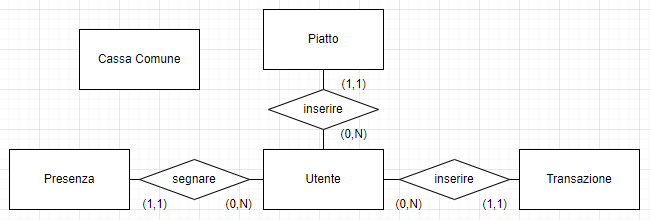
\includegraphics[width=0.9\columnwidth]{database} 
    \caption{Il database progettato per l'applicazione}
    \label{fig:database}
\end{figure}
\newline
Lavorando con Firebase, un database noSQL, i dati sono stati gestiti in modo leggermente diverso, ma rimanendo fedeli alle entità riportate in Figura \ref{fig:database}.\newline
Questo perchè Firebase organizza i dati in \emph{raccolte}, ogni raccolta contiene dei \emph{documenti} e ogni documento è composto da \emph{campi}.\newline
Se dovessimo tradurre a livello teorico:
\begin{itemize}
    \item le \emph{raccolte} sono le entità;
    \item i \emph{documenti} sono le \emph{tuple}, cioè se dovessimo rappresentare le entità come una tabella, un documento è una riga di informazioni dell'entità;
    \item i \emph{campi} sono gli attributi, ovvero un singolo dato della \emph{tupla}.
\end{itemize}
Con Firebase si possono gestire i dati in modo diverso da quanto descritto, perchè i \emph{documenti} non sono rigidi, cioè i \emph{documenti} all'interno di una \emph{raccolta} possono avere quantità e tipi diversi di \emph{campi}, permettendo una struttura dinamica e lasciando al programmatore la libertà di decidere come gestire le informazioni.\newline
\newline
Per convenzione, è stato deciso di strutturare i dati come è stato descritto nell'elenco puntato, perchè risultava più semplice capire l'ordine delle informazioni e ha permesso una semplice gestione dei dati a livello di codice.\newline
Di seguito si riporta la struttura finale del database, riportando per ogni \textbf{raccolta} i \emph{campi} che ogni documento deve contenere.\newline

\newpage

\textbf{cassaComune}
\begin{itemize}
    \item \emph{cassaComune}, di tipo number (numerico)
    \item \emph{quotaPasti}, di tipo number
    \item \emph{quotaStornataStagisti}, di tipo number
\end{itemize}
Per questa raccolta esiste un solo \emph{documento} con codice identificativo "cassaComune".\newline

\textbf{utenti}
\begin{itemize}
    \item \emph{email}, di tipo string (stringa)
    \item \emph{nome}, di tipo string
    \item \emph{cognome}, di tipo string
    \item \emph{UID}, di tipo string; questo rappresenta il codice UID Satispay dell'utente
    \item \emph{quotaStornta}, di tipo string
    \item \emph{admin}, di tipo boolean (booleano)
\end{itemize}

\textbf{piatti}
\begin{itemize}
    \item \emph{nome}, di tipo string
    \item \emph{ingredienti}, di tipo string
    \item \emph{ricetta}, di tipo string
    \item \emph{propostoOggi}, di tipo timestamp; questo permette di capire quando è stata l'ultima volta che il piatto è stato proposto; se riporta la data odierna, il piatto dovrà comparire nella Home
    \item \emph{utente}, di tipo string; serve per capire quale utente ha inserito il piatto
\end{itemize}

\textbf{presenze}
\begin{itemize}
    \item \emph{data}, di tipo timestamp
    \item \emph{utente}, di tipo string
    \item \emph{quotaPasto}, di tipo number; indica quanto riportava la \emph{\gls{quotapastog}} il giorno in cui l'utente è stato presente a pranzo
    \item \emph{stagisti}, di tipo boolean; se impostato a \emph{true} vuol dire che la presenza indicata riporta la presenza degli stagisti e non dell'utente
    \item \emph{numStagisti}, di tipo number; se \emph{stagisti} è impostato a \emph{true} riporta quanti stagisti erano presenti nella data indicata
\end{itemize}
\newpage
\textbf{transazioni}
\begin{itemize}
    \item \emph{soldi}, di tipo number
    \item \emph{data}, di tipo timestamp
    \item \emph{utente}, di tipo sting
    \item \emph{stagista}, di tipo boolean; indica se è stato lo stgista ad effettuare la spesa (\emph{true}) o l'utente (\emph{false})
    \item \emph{spesa}, di tipo boolean; se \emph{true} indica che la transazione riportata è una spesa, altrimenti si tratta dell'invio dei soldi ad un altro utente
    \item \emph{utenteRiceveInvioSoldi}, di tipo string; se \emph{spesa} è impostato a \emph{false}, questo riporta l'utente che riceve i soldi
\end{itemize}

\newpage

%\section{Design Pattern utilizzati}
%forse parlare dell'MVVM o BLoC patttern

\section{Codifica} %riportare qui il database?
%In questa sezione riporto la struttura della cartella lib, parlerò delle componenti e, del file firebase_option e delle classi
%riportare anche le immagine dell'app creata

\subsection{Struttura delle cartelle}
Per il progetto è stato installato il \emph{\gls{sdk}}\glsfirstoccur di Flutter nella versione 3.13.6.\newline  
\newline
La prima cosa che si nota quando si crea un progetto Flutter, è la struttura preimpostata dal \emph{framework} (Figura \ref{fig:directory-flutter}):
\begin{itemize}
    \item all'interno del file \emph{.metadata} si trovano le proprietà del codice Flutter; questo file \textbf{non} bisogna modificarlo perchè contiene i metadati del progetto;
    \item il file \emph{analysis\textunderscore options.yaml} serve per analizzare il codice Dart e controllare che non ci siano errori quando si compila il codice; come è intuibile, anche questo file \textbf{non} bisogna toccarlo;
    \item il file principale che controlla le librerie da installare è \emph{pubspec.yaml}; se si desidera aggiungere un pacchetto, impostare un font specifico o anche indicare la cartella dove bisogna reperire i video e le immagini, bisogna indicarli dentro a questo file;
    \item per ogni piattaforma (Android, iOS, Linux, MacOS, Web e Windows), è presente una cartella apposita con all'interno tutto l'occorente per far funzionare il progetto nel sistema operativo desiderato;
    \item il codice principale lo si scrive all'interno della cartella \emph{lib};
    \item Flutter preimposta la cartella \emph{test} dove poter svolgere i test di unità.
\end{itemize}
\begin{figure}[!h] 
    \centering 
    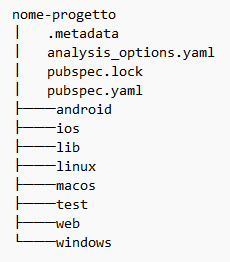
\includegraphics[width=0.35\columnwidth]{FlutterStructure} 
    \caption{La struttura del progetto preimpostata da Flutter}
    \label{fig:directory-flutter}
\end{figure}
Per questo progetto, ho lavorato principalmente nella cartella \emph{lib} e ho creato una cartella \emph{assets} per inserire il logo dell'azienda RiskAPP, visibile nella pagine Acccedi e Registrati dell'app (se fossero state presenti altre immagini, sarebbero state inserite all'interno di questa cartella).\newline
Poche volte ho toccato le cartelle \emph{android} e \emph{ios}, principalmente per sistemare qualche libreria di Flutter che dava problemi su uno dei due sistemi operativi. 
\newpage
\begin{figure}[!h] 
    \centering 
    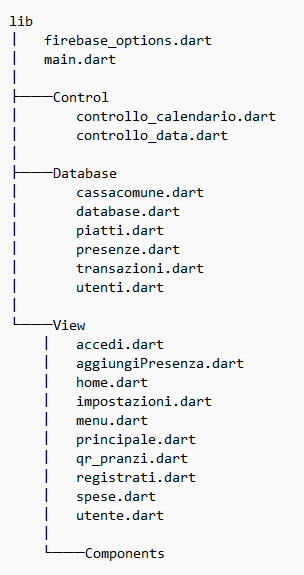
\includegraphics[width=0.45\columnwidth]{libDirectory} 
    \caption{La struttura della cartella lib}
    \label{fig:directory-lib}
\end{figure}
Come si può vedere in Figura \ref{fig:directory-lib}, ho creato tre cartelle per suddividere i file:
\begin{itemize}
    \item nella cartella \textbf{Control}, sono state definite le classi per poter gestire le variabili locali dell'app, che sono solo di supporto per poter gestire alcune informazioni, come per esempio impostare la data nel formato italiano, implementato nella classe ControlloData() creata nel file \emph{controllo\textunderscore  data.dart};
    \item all'interno di \textbf{Database}, sono presenti tutte le classi con le funzioni appropriate per poter comunicare e gestire il database di Firebase;
    \item all'interno della cartella \textbf{View}, viene gestita la parte grafica dell'app; per ogni pagina è stata creato un file apposito, l'unica eccezione è per \emph{principale.dart} che ha il solo scopo di visualizzare la barra inferiore dell'app.
\end{itemize}
Il file \emph{firebase\textunderscore options.dart} contiene le istruzioni fondamentali per collegare il progetto alla console di Firebase e viene generato automaticamente da \emph{FlutterFire \gls{clig}\glsfirstoccur}, un tool che mette a disposizione diversi comandi per installare \emph{FlutterFire} e permettere di collegare il proprio progetto a Firebase.\newline
In \emph{main.dart} si decide quale pagina deve visualizzare l'utente quando apre l'app, in base se è stato eseguito l'accesso le volte precedenti o no.
%\newpage
\begin{figure}[!h] 
    \centering 
    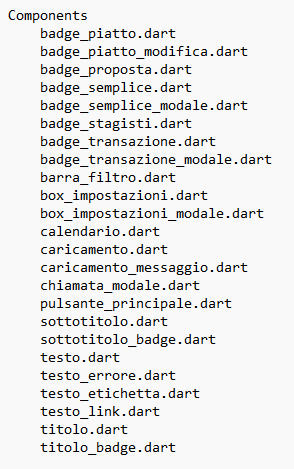
\includegraphics[width=0.45 \columnwidth]{ComponentsDirectory} 
    \caption{La struttura della cartella Components}
    \label{fig:directory-components}
\end{figure}

In \textbf{View} è presente la cartella \textbf{Components} (Figura \ref{fig:directory-components}), questa contiene le componenti, ovvero degli elementi preimpostati che vengono utilizzati più volte all'interno del codice.\newline
Per esempio, il file \emph{caricamento.dart} definisce la schermata che dovrà essere visibile mentre viene eseguito un caricamento dei dati da Firebase; questo componente viene richiamato da quasi tutte le pagine create in \textbf{View}.

\newpage

\subsection{Le librerie di Firebase}
Quando si collega un progetto a Firebase, si scaricano i pacchetti \emph{Firebase \gls{clig}} e \emph{FlutterFire \gls{clig}}, questi permettono di collegare il progetto alla console di Firebase e creano il file \emph{firebase\textunderscore option.dart} che dovrà poi essere importato nel file \emph{main.dart}.\newline
Infine, basta scrivere le righe di codice riporte in Figura \ref{fig:code-firebase} per poter permettere ad ogni piattaforma di interagire con il database.
\begin{figure}[!h] 
    \centering 
    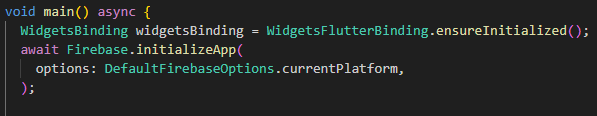
\includegraphics[width=0.95 \columnwidth]{code/firebase} 
    \caption{Istruzione per collegare Firebase}
    \label{fig:code-firebase}
\end{figure}

Quando si eseguono i passaggi appena descritti, si installa in automatico il pacchetto \emph{firebase\textunderscore core}, ma per poter permettere l'autenticazione degli utenti e lavorare con il database, sono stati installati manualmente i pacchetti \emph{firebase\textunderscore auth} e \emph{cloud\textunderscore firestore}.\newline
\newline
Ci sono diversi modi che Firebase Authentication mette a disposizione per la registrazione di un utente, ma per questo progetto è stato adottato il metodo di autenticazione tramite mail e password.\newline
Per permettere la registrazione, l'accesso e la disconnessione di un utente, è stato creata la classe \emph{Database} che al suo interno contiene solo i metodi con le funzioni appena descritte (in Figura \ref{fig:code-authentication} sono riportate le funzioni \emph{accedi} e \emph{disconettiti}).
\begin{figure}[!h] 
    \centering 
    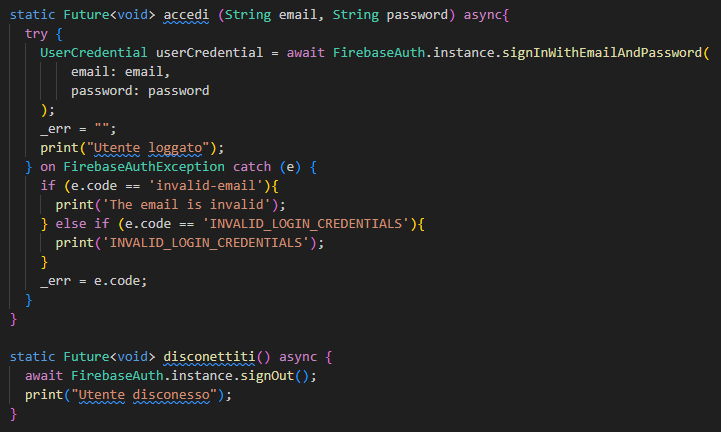
\includegraphics[width=1.05 \columnwidth]{code/firebaseauth} 
    \caption{Le funzioni di accesso e di disconnesione di un utente}
    \label{fig:code-authentication}
\end{figure}

\newpage

Per poter lavorare con il Cloud di Firestore, è stata creata una classe per ogni entità.\newline
Ogni classe contiene un metodo per creare una nuova istanza (Figura \ref{fig:code-aggiungi}), metodi \emph{set} e \emph{get} per ogni campo (Figura \ref{fig:code-query}) e alcune funzioni di supporto.
\begin{figure}[!h] 
    \centering 
    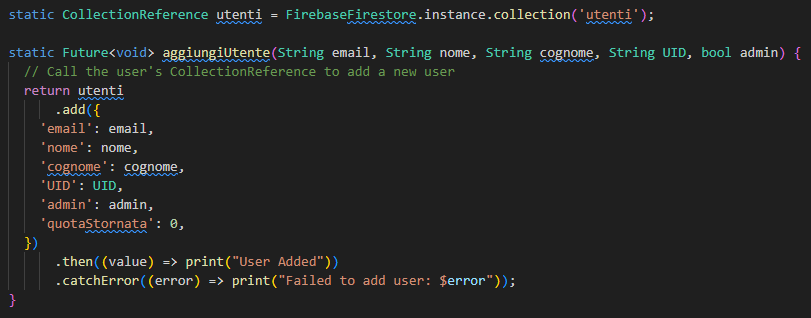
\includegraphics[width=1.1 \columnwidth]{code/aggiuntautente} 
    \caption{La funzione di aggiunta di un utente nel database}
    \label{fig:code-aggiungi}
\end{figure}
\begin{figure}[!h] 
    \centering 
    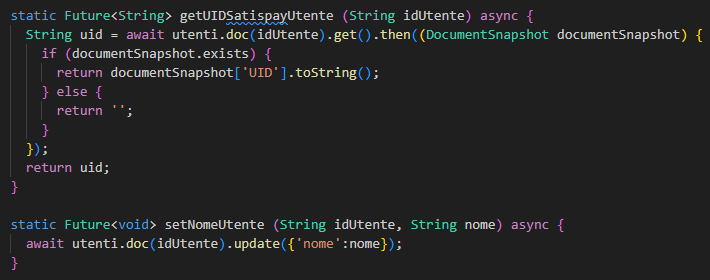
\includegraphics[width=1.00 \columnwidth]{code/query-set} 
    \caption{Una funzione \emph{get} e \emph{set} della classe \emph{Utenti}}
    \label{fig:code-query}
\end{figure}

Attraverso la console di Firebase è possibile vedere gli utenti che si sono registrati, i dati presenti nel database ed è possibile anche modificare i permessi di lettura o modifica dei dati, per un controllo più attento anche a livello di codice. 

\newpage

\subsection{Il calendario delle presenze}
Per permettere la gestione delle presenze, è stato installato il pacchetto \emph{table\textunderscore calendar}, che permette di creare il \emph{widget} TableCalendar, cioè l'elemento grafico che vediamo in Figura \ref{fig:calendario}.
\begin{figure}[!h] 
    \centering 
    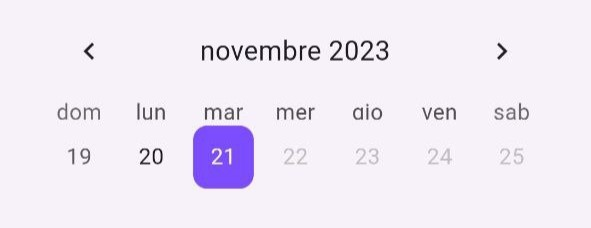
\includegraphics[width=0.5 \columnwidth]{calendario} 
    \caption{Il calendario che l'utente utilizza per gestire le presenze}
    \label{fig:calendario}
\end{figure}

Il \emph{widget} offre una serie di opzioni che consentono di modificarlo, come per esempio scegliere se visualizzare il calendario nel formato settimanale (come in immagine), con due settimane oppure tutto un mese.\newline
Si può modificare come viene visualizzata la data selezionata (anche la data odierna) attraverso l'uso del \emph{CalendarBuilder}: si tratta di un costruttore (\emph{builder}) con il compito di impostare la grafica dell'elemento indicato; in questo caso ha il compito di impostare la grafica delle date evidenziate.\newline
\newline
Questo calendario è presente nella pagina Utente, dove sono visibili i tre \emph{widget} grigi, il primo apre il calendario per modificare le proprie presenze (Figura \ref{fig:utente-presenze}), il secondo, visibile per gli amministratori, apre il calendario per modificare e monitorare le presenze degli stagisti.\newline
Il terzo \emph{widget} consente solo di visualizzare e modificare la \emph{\gls{quotapastog}}.\newline
Non sono stati inseriti altri calendari nell'applicazione.\newline
\newline
Una funzione fondamentale di TableCalendar è \emph{onDaySelected}: questa permette di modificare il calendario selezionato, rendendo la selezione iterativa; se non viene definita questa funzione, il calendario rimane statico e non sarà possibile cambiare la data selezionata, ma rimarrà evidenziata la data indicata inizialmente nella variabile \emph{focusedDay}.
\newpage
\begin{figure}[!h] 
    \centering 
    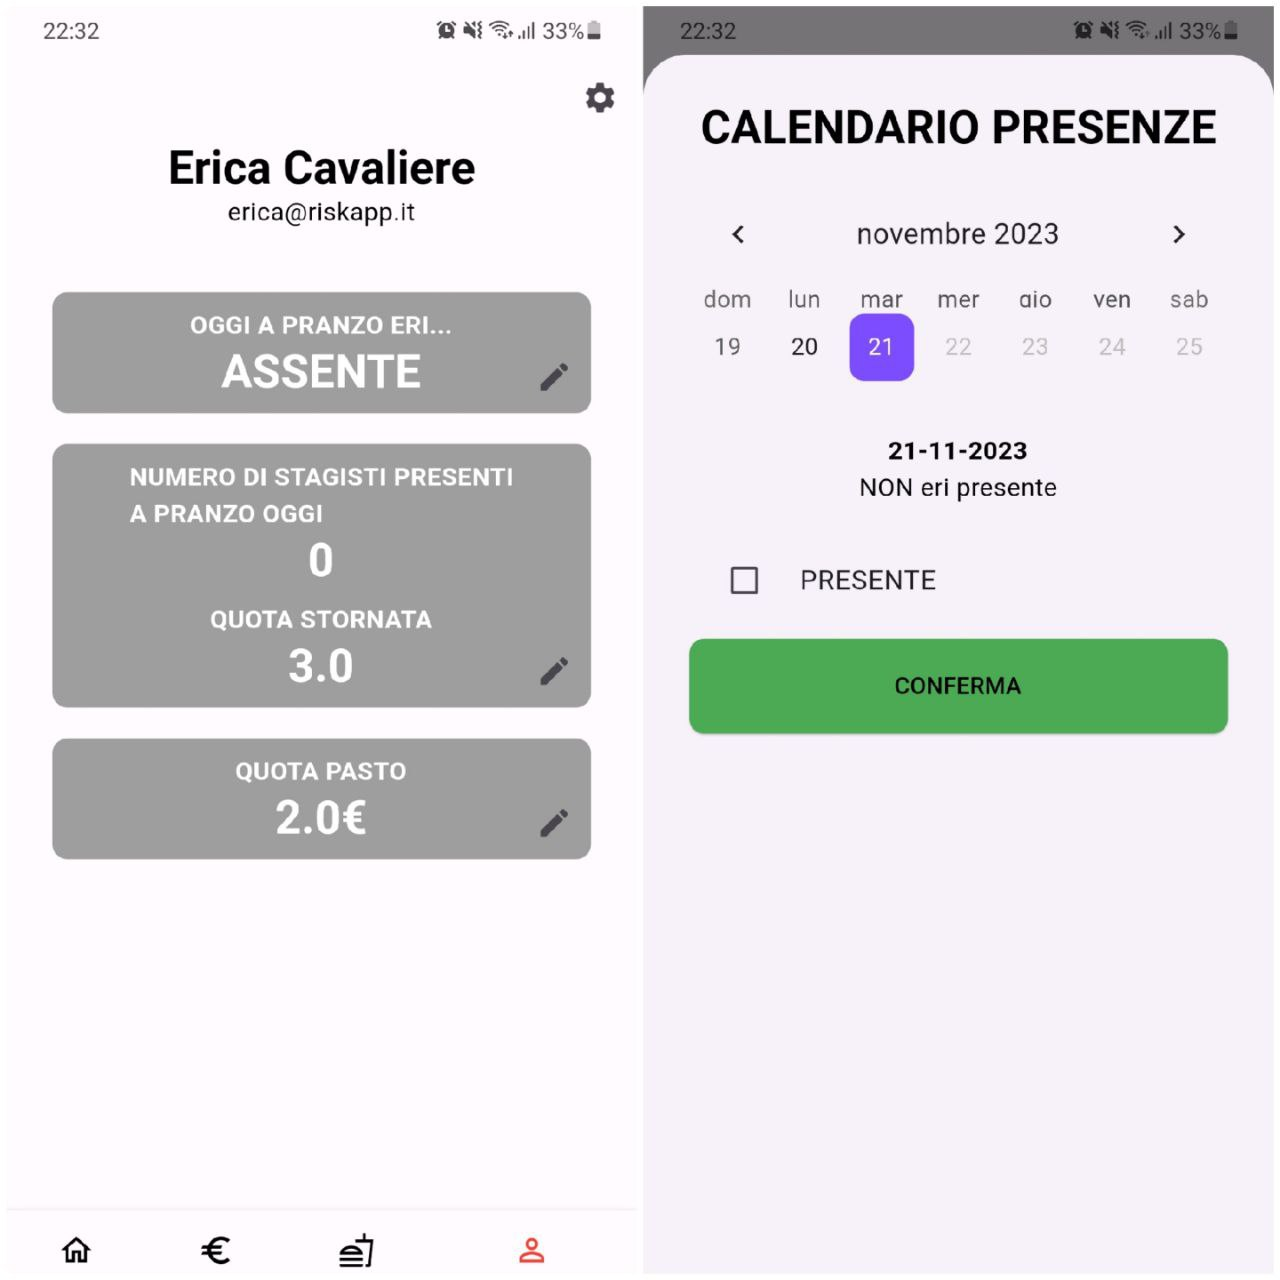
\includegraphics[width=0.7 \columnwidth]{Utente} 
    \caption{La schermata Utente e il calendario delle presenze}
    \label{fig:utente-presenze}
\end{figure}
\begin{figure}[!h] 
    \centering 
    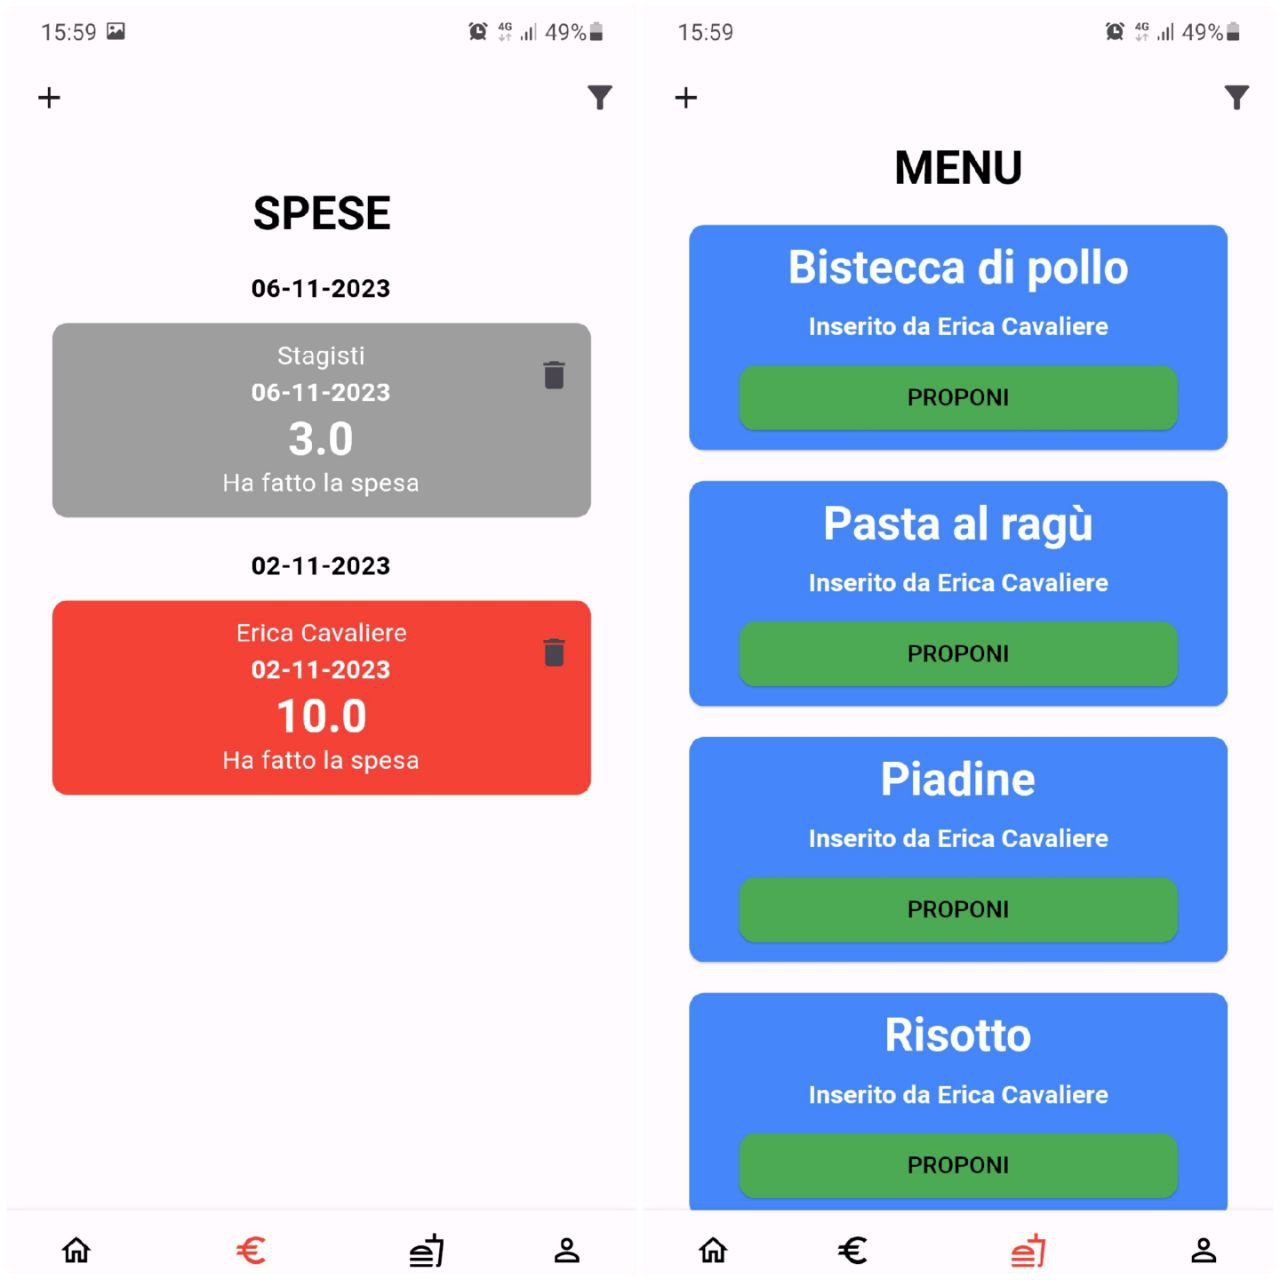
\includegraphics[width=0.7 \columnwidth]{SpeseMenu} 
    \caption{Le schermate Spese e Menu}
    \label{fig:spese-menu}
\end{figure}
\newpage

\subsection{Altre schermate dell'app}
Per questo progetto è stata richiesta un'app che permettesse, oltre un controllo e una gestione delle presenze, anche un controllo delle spese e la presenza di un menu comune per tutti, dove è possibile proporre un piatto per il pranzo odierno (Figura \ref{fig:spese-menu}).\newline
Tramite la barra superiore di entrambe le schermate, è possibile aggiungere un elemento alla lista oppure utilizzare il filtro per visualizzare solo alcuni elementi specifici.\newline
\newline
Quando si effettua una aggiunta o si applica un filtro, il lavoro che l'app svolge è aggiornare il database o richiedere degli elementi specifici nel cloud di Firebase, per poi aggiornare graficamente la lista interessata.\newline
Ogni modifica in Firebase, viene ripotata in tempo reale su tutti i dispositivi che utilizzano l'app; per permettere questo, sono stati utilizzati gli \textbf{StreamBuilder} (\cite{site:flutter-streambuilder}).\newline
Dato uno \emph{stream} di dati, lo \textbf{StreamBuilder} si occupa di creare e aggiornare dei \emph{widget} specifici, in questo caso si occupa di aggiornare le liste presenti nelle schermate Spesa e Menu.\newline
\newline
Lo \textbf{StreamBuilder} è stato utilizzato anche nella Home, per permettere all'utente di monitorare in tempo reale i piatti proposti, la \emph{\gls{cassacomuneg}} e la propria \emph{\gls{quotastornatag}}, quest'ultimi due sono in continuo aggiornamento in base alle modifiche riportate nella schermata Spese o tramite le presenze segnate nel calendario (per ogni presenza viene effettuata una modifica pari alla quantità di soldi indicata nella \emph{\gls{quotapastog}}).\newline
È stato utilizzato lo \textbf{StreamBuilder} anche nella schermata Utente per il controllo in tempo reale della \emph{\gls{quotastornatag}} degli stagisti.

\newpage

\subsection{Modificare il nome e il logo}
Quando si crea un'applicazione, di default Flutter imposta il suo logo.\newline
Per poter modificare e utilizzare il proprio logo è molto semplice, prima di tutto bisogna creare più formati dell'immagine che si desidera attribuire all'app, poi bisogna riportarli tutti all'interno della cartella del sistema operativo interessato e preimpostato da Flutter.
\begin{itemize}
    \item Per Android bisogna salvare il logo e tutti i suoi formati nel percorso\newline andorid/app/src/main/res
    \item Per iOS bisogna salvare il logo e tutti i suoi formati nel percorso\newline ios/Runner/Assets.xcassets/AppIcon.appiconset
\end{itemize}
Il logo per questo progetto è stato creato in Figma (Figura \ref{fig:logo-nome}).\newline
\newline
Il procedimento per modificare il nome dell'applicazione non si discosta molto dal procedimento appena descritto.
\begin{itemize}
    \item Per Android bisogna modificare il parametro \emph{label} presente nel file\newline \emph{AndroidManifest.xml} che si trova nel percorso andorid/app/src/main.
    \item Per iOS bisogna modificare il parametro \emph{CFBundleDisplayName} nel file \emph{Info.plist} presente nel percorso ios/Runner.
\end{itemize}
\begin{figure}[!h] 
    \centering 
    
\includegraphics[width=0.2 \columnwidth]{GestionePranzi} 
    \caption{Il nome e il logo dell'applicazione creata}
    \label{fig:logo-nome}
\end{figure}

\newpage

\subsection{Aprire l'app tramite QrCode}